\documentclass{beamer}

\mode<presentation>
{
  \usetheme{CambridgeUS}      % or try Darmstadt, Madrid, ...
  \usecolortheme{default} % or try albatross, beaver, crane, ...
  \usefonttheme{default}  % or try serif, structurebold, ...
  \setbeamertemplate{navigation symbols}{}
  \setbeamertemplate{caption}[numbered]
} 

\usepackage[english]{babel}
\usepackage[utf8x]{inputenc}
\usepackage{listings}
\usepackage[ampersand]{easylist}



\definecolor{KTI_green}{RGB}{150, 189, 13}
\definecolor{TU_red}{RGB}{255, 55, 81}
\definecolor{faint_gray}{RGB}{180, 180, 180}

\definecolor{syntax_green}{rgb}{0,0.6,0}
\definecolor{syntax_gray}{rgb}{0.9, 0.9, 0.9}
\definecolor{syntax_mauve}{rgb}{0.58,0,0.82}

\lstset{ 
  backgroundcolor=\color{syntax_gray},  % choose the background color
  basicstyle=\scriptsize\ttfamily,        		% size of fonts used for the code
  breaklines=false,                		% automatic line breaking only at whitespace
  captionpos=b,                    		% sets the caption-position to bottom
  commentstyle=\color{syntax_green},    % comment style
  escapeinside={\%*}{*)},          		% if you want to add LaTeX within your code
  keywordstyle=\color{blue},       		% keyword style
  stringstyle=\color{syntax_mauve},     % string literal style
  columns=fullflexible,
  frame=single,
  framesep=0.5cm,
  framexleftmargin=0.5cm,
  xleftmargin=0.5cm,
  framexrightmargin=0.5cm,
  xrightmargin=0.5cm,
  frame=tb,                 
    numbers=left,                    
    numbersep=15pt,  
  }
  
  
\newcommand{\logopython}{\raggedleft 
\includegraphics[height=0.5cm]{logo_python}\hspace{0.1cm}\\\raggedright}
\newcommand{\logopythonbottom}{\raggedleft\vspace{-0.8cm}
\includegraphics[height=0.5cm]{logo_python}\hspace*{0.05cm}\\\raggedright}

\title[BSP03 - Sortierung ZZ]{Sortierung von Zufallszahlen}
\author{Dickbauer Y., Moser P., Perner M.}
\institute{PS Computergestützte Modellierung, WS 2016/17}
%\date{Date of Presentation}

\begin{document}

\begin{frame}
  \titlepage
\end{frame}

% Uncomment these lines for an automatically generated outline.
\begin{frame}{Outline}
  \tableofcontents
\end{frame}

\section{Aufgabenstellung}
\begin{frame}{Aufgabenstellung}

\begin{itemize}
  \item Eingabe: Anzahl an n Zufallszahlen
  \item Erstellung von n Zufallszahlen
  \item Erstellung einer Liste dieser generierten Zufallszahlen
  \item Sortierung dieser Liste Aufsteigend. 1. Priorität nach X, \\2. Priorität: Y
  \item Ausgabe der Liste
\end{itemize}

\end{frame}

\section{Flow Chart}
\begin{frame}{Flow Chart}
	\centering
  	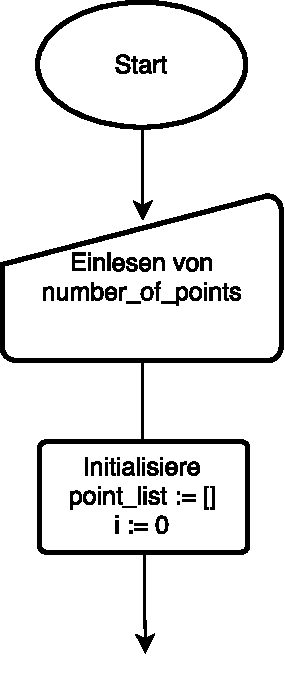
\includegraphics[scale=0.4]{BSP03_Flow_Chart_1.pdf}
\end{frame}
\begin{frame}{Flow Chart}
	\centering
  	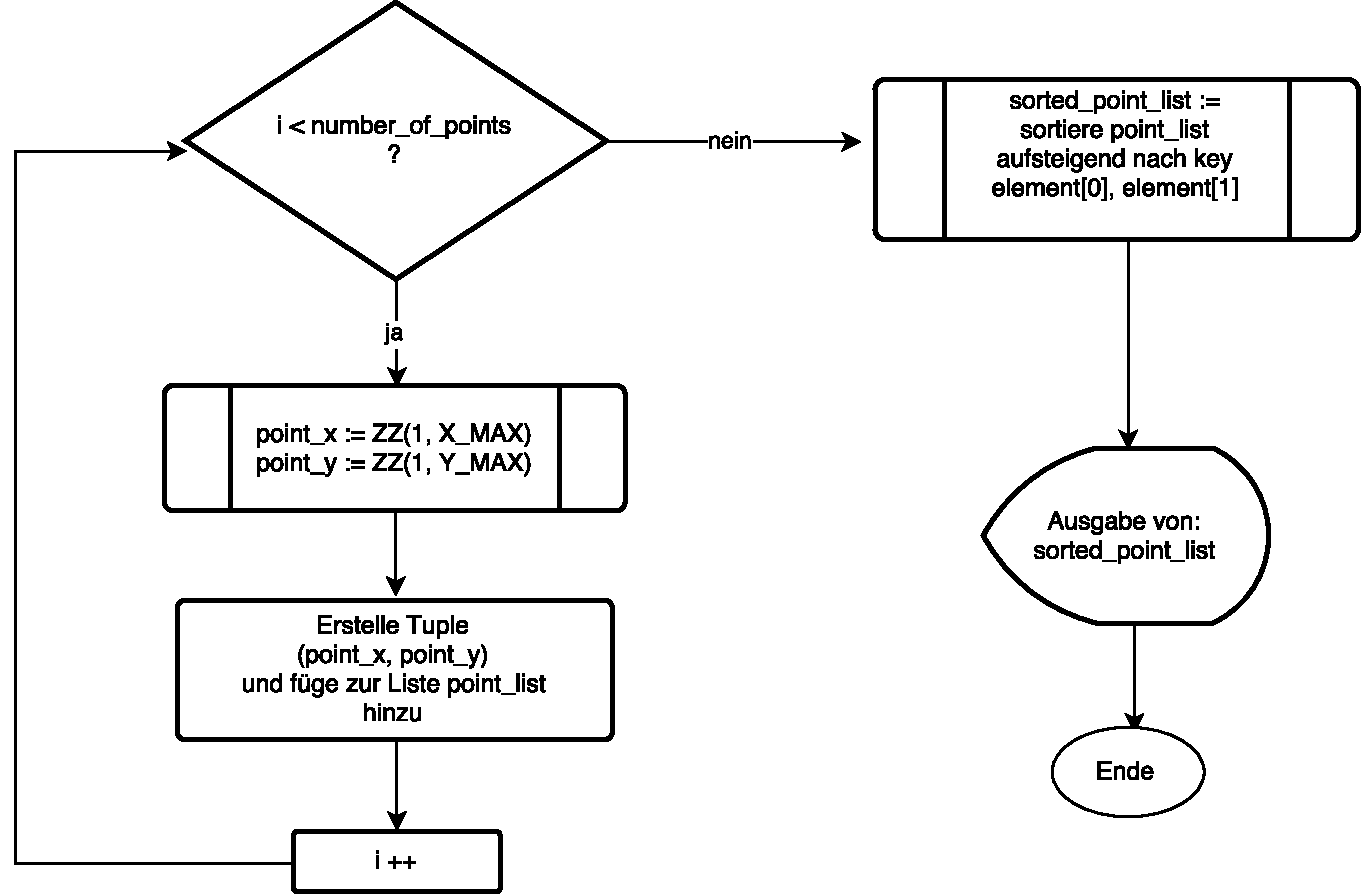
\includegraphics[scale=0.4]{BSP03_Flow_Chart_2.pdf}
\end{frame}

\section{Programmcode}
\subsection{Main Funktion}
\begin{frame}[fragile]{Main Funktion - Programmeinstieg}
  \begin{lstlisting}[language=python]
def main():
    # user input:
    inp = user_input((
        ('Number of points', int, 10),), DEBUG)
    number_of_points = inp[0]
    
    # generate points:
    point_list = []
    for i in range(number_of_points):
        point_x = random_number_from_interval(1, X_MAX)
        point_y = random_number_from_interval(1, Y_MAX)
        point = (point_x, point_y)
        point_list.append(point)
        
    # sort
    sorted_point_list = sorted(point_list, key=sort_key_function)
    
    # output
    for x, y in sorted_point_list:
        print('x: {:5f}\ty: {:5f}'.format(round(x, 2), round(y, 2)))
\end{lstlisting}
\logopythonbottom
\end{frame}

\subsection{Verwendete Funktionen}
\begin{frame}[fragile]{Funktion random\_number\_from\_interval(..)}
  \begin{itemize}
    \item Diese Funktion verlangt zwei Eingabeparameter \textit{lower} und \textit{upper}
    \item Gibt eine (pseudo)Zufallszahl (\textit{float}) im Intervall  [\textit{lower}, \textit{upper}) zurück 
    \item \textit{random.random()} ist eine Funktion der Python Standardbibliothek, welche ein Zufallszahl (\textit{float}) im Intervall [\textit{lower}, \textit{upper}) zurück gibt
    \item Mersenne Twister Methode wird als Generator der ZZ verwendet\footnote[frame] {\scriptsize\url{https://docs.python.org/3.5/library/random.html}} \footnote[frame] {\scriptsize\url{https://en.wikipedia.org/wiki/Mersenne_Twister}}
  \end{itemize}
  \begin{lstlisting}[language=python]
def random_number_from_interval(lower, upper):
    val = random.random()
    return lower + (upper -lower) * val
\end{lstlisting}
\logopythonbottom
\end{frame}	
\begin{frame}[fragile]{Funktion user\_input(input\_vars, [use\_defaults])}
  \begin{itemize}
  	\item Diese Funktion verlang vom User die geforderten Eingabeparameter und gibt diese als von der Programmiererin gewünschten Datentyp wieder zurück
    \item Funktion verlangt als ersten Eingabeparameter die Liste \textit{input\_vars}
    \item Falls \textit{use\_defaults == True} wird der User nicht nach Eingabe gefragt (Dient zum Testen)
    \item Diese Liste besteht wiederrum aus Listen mit je Länge = 3:
    \begin{itemize}
    	\item 0: Text, welcher dem User ausgegeben wird
    	\item 1: Datentyp (int/float/str)
    	\item 2: Default value: Dieser Wert wird zurueckgegeben, falls \textit{use\_defaults == True}
    \end{itemize}
  \end{itemize}
  \begin{lstlisting}[language=python]
x, y = user_input((
    ('Geben Sie einen X Wert ein', int, 10),
    ('Geben Sie einen Y Wert ein', int,  5), False):
  \end{lstlisting}
  \logopythonbottom
\end{frame}	

\section{Beispiel}
\begin{frame}{Beispiel anhand fixer Zufallszahlen}
\begin{itemize}
\item X\_MAX = 10, Y\_MAX = 10
\item Usereingabe: number\_of\_points := 8
\item Annahme der Zufallszahlen wie folgt:
\end{itemize}
\begin{center}
  \begin{tabular}{c|c|c|c|c|c|c|c|c|c}
  \hline 
  i & 0 & 1 & 2 & 3 & 4 & 5 & 6 & 7 & 8 \\ 
  \hline 
  ZZ fuer X & 5 & 2 & 5 & 3 & 3 & 9 & 1 & 7 & 3\\ 
  ZZ fuer Y & 9 & 7 & 8 & 4 & 3 & 1 & 7 & 2 & 1\\
  \hline 
  \end{tabular} 
\end{center}
\end{frame}

\begin{frame}[fragile]{Beispiel anhand fixer Zufallszahlen}
For-Schleife zum Erzeugen der point\_list:
\begin{easylist}
\ListProperties(Hide=100, Hang=true, Progressive=3ex, Style*= ,
Style2*=$\bullet$ ,Style3*=$\circ$ ,Style4*=\tiny$\blacksquare$ )
& i := 0
&& point\_x := 5, point\_x := 9 
&& point\_list := [(5,9)]
& i := 1
&& point\_x := 2, point\_x := 7 
&& point\_list := [(5,9), (2,7)]
& i := 2
&& point\_x := 5, point\_x := 8 
&& point\_list := [(5,9), (2,7), (5,8)]
& ...
& i := 8
&& point\_x := 3, point\_x := 1 
&& point\_list := [(5,9),(2,7),(5,8),(3,4),(3,3),(9,1),(1,7),(7,2),(3,1)]
\end{easylist}
\end{frame}

\begin{frame}[fragile]{Beispiel anhand fixer Zufallszahlen}
Sortieren der point\_list:
\begin{easylist}
\ListProperties(Hide=100, Hang=true, Progressive=3ex, Style*=-- ,
Style2*=$\bullet$ ,Style3*=$\circ$ ,Style4*=\tiny$\blacksquare$ )
& point\_list hat nun die Länge 8 mit je (x,y) Tuples als Eintrag
& sorted() ist eine built-in Funktion, welche einen \textit{key} benötigt, um zu wissen, wie sie die Listeneinträge sortieren soll
&& Als Key wird nun einfach (x,y) gegeben, das Sortieren geht nun automatisch aufsteigend zuerst nach x, danach nach y (comperator gibt es in python ab Version 3 nicht mehr)\footnote[frame] {\scriptsize\url{https://docs.python.org/3.5/library/functions.html\#sorted}}
&& Alternativlösung: Zuerst nach key y sortieren, danach nach x
& sorted\_point\_list :=
&& [(1,7), (2,7), (3,3), (3,4), (5,8), (5,9), (7,2), (9,1)]
\end{easylist}
\end{frame}

\begin{frame}[fragile]{Anhang: Modifikation des Source Codes um Demo Beispiel zu erhalten}
  \begin{lstlisting}[language=python]
  # Aendere random_number_from_interval() in lib.py wie folgt:
ZZ = [5,9,2,7,5,8,3,4,3,3,9,1,1,7,7,2,3,1]
i = -1
def random_number_from_interval(lower, upper):
    global i
    i += 1
    return ZZ[i]
  \end{lstlisting}
\logopythonbottom
\end{frame}
\end{document}
